\section{pbdR}
\makesubcontentsslides

\subsection{The pbdR Project}
\makesubcontentsslidessec

\begin{frame}{\pbdR Interfaces to Libraries: Sustainable Path}
  \vspace{-1ex}
  \centering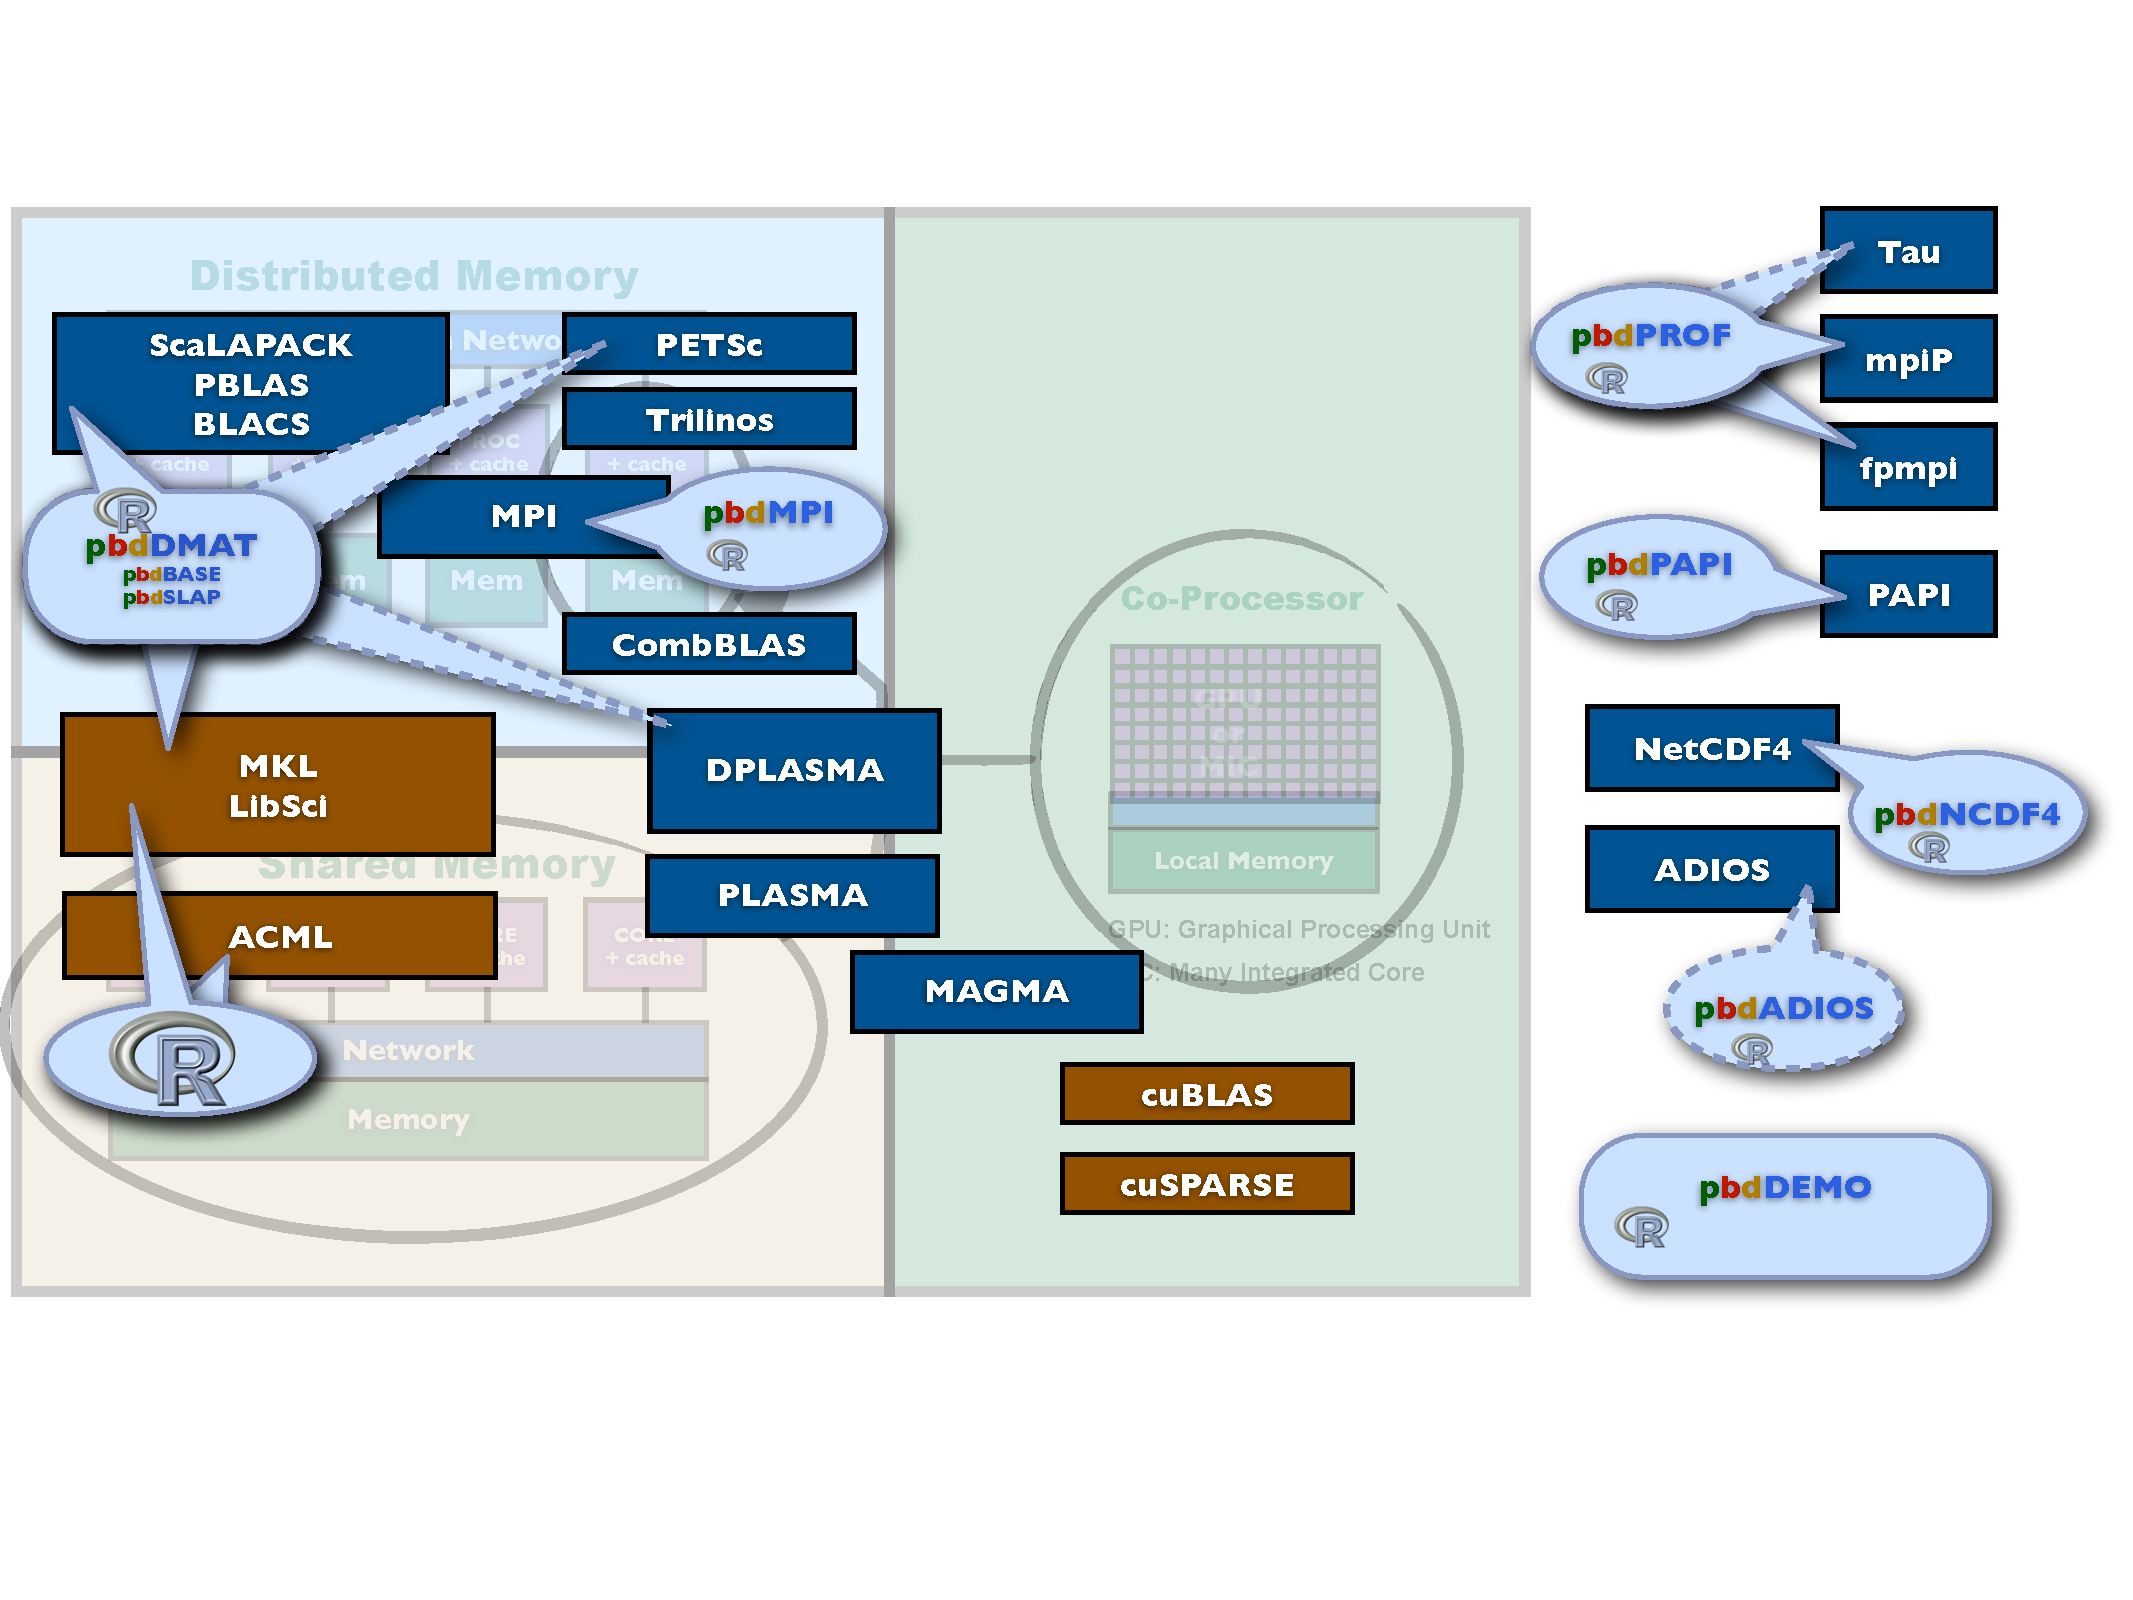
\includegraphics[trim=0cm 5cm 0cm 3cm,clip=true,width=0.85\textwidth]
  {../common/pics/hardware/ParallelHardware27.pdf}
  \scriptsize
  \begin{block}{Why use HPC libraries?}
    \begin{itemize}[<+-|alert@+>]
    \item The libraries represent 30+ years of research by the HPC
      community
    \item \emph{They're tested.} \emph{They're
        fast.}  \emph{They're scalable.}
    \item Many science communities are invested in their API.
    \item HPC Simulation Science uses much of the same math as data
      analysis
    \end{itemize}
  \end{block}
\end{frame}

\subsection{pbdMPI}
\makesubcontentsslidessec

\begin{frame}
  \begin{block}{pbdMPI: Simplified, Extensible, and Fast Communication Operations}\pause
    \begin{itemize}
    \item S4 methods for collective communication: extensible to other
      \R objects.
    \item Default methods (like \code{Robj} in \pkg{Rmpi}) check for
      data type: safe for general users.
    \item API is simplified: defaults in control objects.
    \item Array and matrix methods without serialization: faster than
      \pkg{Rmpi}.
    \end{itemize}
    \begin{center}
      \vspace{0.2cm}\scriptsize
      \begin{tabular}{ll} \hline\hline
        \pkg{pbdMPI} (S4) & \pkg{Rmpi}                \\ \hline
        \code{allgather}    & \code{mpi.allgather},
        \code{mpi.allgatherv},
        \code{mpi.allgather.Robj} \\
        \code{allreduce}    & \code{mpi.allreduce}      \\
        \code{bcast}        & \code{mpi.bcast},
        \code{mpi.bcast.Robj}     \\
        \code{gather}       & \code{mpi.gather},
        \code{mpi.gatherv},
        \code{mpi.gather.Robj}    \\
        \code{recv}         & \code{mpi.recv},
        \code{mpi.recv.Robj}      \\
        \code{reduce}       & \code{mpi.reduce}         \\
        \code{scatter}      & \code{mpi.scatter},
        \code{mpi.scatterv},
        \code{mpi.scatter.Robj}   \\
        \code{send}         & \code{mpi.send},
        \code{mpi.send.Robj}      \\ \hline \hline
      \end{tabular}
    \end{center}
  \end{block}
\end{frame}

\begin{frame}[fragile]
  \begin{block}{Integer?\qquad Not always obvious in R.}
    \vspace{-.2cm}
    \begin{lstlisting}
> is.integer(1)
[1] FALSE
> is.integer(2)
[1] FALSE
> is.integer(1:2)
[1] TRUE
    \end{lstlisting}
  \end{block}
  \begin{block}{pbdMPI lets R figure it out}\pause
    \begin{minipage}[t]{.475\textwidth}
      \begin{lstlisting}[title=Rmpi]
# int
mpi.allreduce(x, type=1)
# double
mpi.allreduce(x, type=2)
      \end{lstlisting}
    \end{minipage}
    \hfill
    \begin{minipage}[t]{.475\textwidth}
      \begin{lstlisting}[title=pbdMPI]
allreduce(x)
      \end{lstlisting}
      % \vspace{1em}
      % \hspace{1em}{\small S4. Batch only! (No spawning)}
    \end{minipage}
  \end{block}
\end{frame}


\begin{frame}[fragile]{Single Program (SPMD): Runs Asynchronous Parallel}
  \begin{exampleblock}{Rank Query Example}
    \centering
    \begin{lstlisting}[title=1\_rank.r]
library(pbdMPI, quiet = TRUE)
init()

my.rank <- comm.rank()
comm.print(my.rank, all.rank=TRUE)

finalize()
    \end{lstlisting}
    \begin{columns}[t,onlytextwidth]
      \begin{column}{0.62\textwidth}
        \begin{lstlisting}[backgroundcolor=\color{white},keywordstyle=\color{black},
title=Execute this batch script via:]
mpirun -np 2 Rscript 1_rank.r
        \end{lstlisting}
      \end{column}
      \hfill
      \begin{column}{0.35\textwidth}
        \begin{lstlisting}[title=Sample Output:]
COMM.RANK = 0
[1] 0
COMM.RANK = 1
[1] 1
        \end{lstlisting}
      \end{column}
    \end{columns}
  \end{exampleblock}
\end{frame}

\subsection{pbdDMAT}
\makesubcontentsslidessec

\begin{frame}{Mapping a Matrix to Processors}
  \begin{block}{Processor Grid Shapes}
    \begin{table}[ht]
      \centering
      % \begin{subfigure}[b]{0.23\textwidth}
      %   \centering
      %   $\left[\begin{tabular}{l}
      %       0 \\ 1 \\ 2 \\ 3 \\ 4 \\ 5
      %     \end{tabular}\right]^T$
      %   \caption{$1\times 6$}
      % \end{subfigure}
      \begin{subfigure}[b]{0.23\textwidth}
        \centering
        $\left[\begin{tabular}{llllll}
            0 & 1 & 2 & 3 & 4 & 5
          \end{tabular}\right]$
        \vspace{1.5cm}
        \caption{$1\times 6$}
      \end{subfigure}%\hspace{-1cm}
      \begin{subfigure}[b]{0.23\textwidth}
        \centering
        $\left[\begin{tabular}{lll}
            0 & 1 & 2\\
            3 & 4 & 5
          \end{tabular}\right]$
        \caption{$2\times 3$}
      \end{subfigure}%
      \begin{subfigure}[b]{0.23\textwidth}
        \centering
        $\left[\begin{tabular}{ll}
            0 & 1 \\
            2 & 3\\
            4 & 5
          \end{tabular}\right]$
        \caption{$3\times 2$}
      \end{subfigure}
      \begin{subfigure}[b]{0.23\textwidth}
        \centering
        $\left[\begin{tabular}{l}
            0 \\ 1 \\ 2 \\ 3 \\ 4 \\ 5
          \end{tabular}\right]$
        \caption{$6\times 1$}
      \end{subfigure}
      \caption{Processor Grid Shapes with 6 Processors}\label{fig:gridshapes}
    \end{table}
  \end{block}
\end{frame}

\begin{frame}[shrink]
\begin{exampleblock}{2$\times$3 block-cyclic grid on 6 processors:
    Global view ``ddmatrix'' class}
\begin{align*}
x &= \left[
      \begin{array}{ll|ll|ll|ll|l}
      \color{g11}x_{11} & \color{g11}x_{12} & \color{g12}x_{13} & \color{g12}x_{14} & \color{g13}x_{15} & \color{g13}x_{16} & \color{g11}x_{17} & \color{g11}x_{18} & \color{g12}x_{19}\\
      \color{g11}x_{21} & \color{g11}x_{22} & \color{g12}x_{23} & \color{g12}x_{24} & \color{g13}x_{25} & \color{g13}x_{26} & \color{g11}x_{27} & \color{g11}x_{28} & \color{g12}x_{29}\\\hline
      \color{g21}x_{31} & \color{g21}x_{32} & \color{g22}x_{33} & \color{g22}x_{34} & \color{g23}x_{35} & \color{g23}x_{36} & \color{g21}x_{37} & \color{g21}x_{38} & \color{g22}x_{39}\\
      \color{g21}x_{41} & \color{g21}x_{42} & \color{g22}x_{43} & \color{g22}x_{44} & \color{g23}x_{45} & \color{g23}x_{46} & \color{g21}x_{47} & \color{g21}x_{48} & \color{g22}x_{49}\\\hline
      \color{g11}x_{51} & \color{g11}x_{52} & \color{g12}x_{53} & \color{g12}x_{54} & \color{g13}x_{55} & \color{g13}x_{56} & \color{g11}x_{57} & \color{g11}x_{58} & \color{g12}x_{59}\\
      \color{g11}x_{61} & \color{g11}x_{62} & \color{g12}x_{63} & \color{g12}x_{64} & \color{g13}x_{65} & \color{g13}x_{66} & \color{g11}x_{67} & \color{g11}x_{68} & \color{g12}x_{69}\\\hline
      \color{g21}x_{71} & \color{g21}x_{72} & \color{g22}x_{73} & \color{g22}x_{74} & \color{g23}x_{75} & \color{g23}x_{76} & \color{g21}x_{77} & \color{g21}x_{78} & \color{g22}x_{79}\\
      \color{g21}x_{81} & \color{g21}x_{82} & \color{g22}x_{83} & \color{g22}x_{84} & \color{g23}x_{85} & \color{g23}x_{86} & \color{g21}x_{87} & \color{g21}x_{88} & \color{g22}x_{89}\\\hline
      \color{g11}x_{91} & \color{g11}x_{92} & \color{g12}x_{93} & \color{g12}x_{94} & \color{g13}x_{95} & \color{g13}x_{96} & \color{g11}x_{97} & \color{g11}x_{98} & \color{g12}x_{99}\\
      \end{array}
\right]_{9\times 9}
\end{align*}
\begin{align*}
\text{Processor grid = }\left|
      \begin{array}{lll}
      \color{g11}0 & \color{g12}1 & \color{g13}2\\
      \color{g21}3 & \color{g22}4 & \color{g23}5
      \end{array}
\right| &=
\left|
      \begin{tabular}{lll}
      \color{g11}(0,0) & \color{g12}(0,1) & \color{g13}(0,2)\\
      \color{g21}(1,0) & \color{g22}(1,1) & \color{g23}(1,2)
      \end{tabular}
\right|
\end{align*}
\end{exampleblock}
\end{frame}


\begin{frame}[shrink]
\begin{exampleblock}{2$\times$3 block-cyclic grid on 6 processors:
    Local view ``ddmatrix'' class}
\begin{align*}
\left[
      \begin{array}{ll|ll}
      \color{g11}x_{11} & \color{g11}x_{12} & \color{g11}x_{17} & \color{g11}x_{18}\\
      \color{g11}x_{21} & \color{g11}x_{22} & \color{g11}x_{27} & \color{g11}x_{28}\\\hline
      \color{g11}x_{51} & \color{g11}x_{52} & \color{g11}x_{57} & \color{g11}x_{58}\\
      \color{g11}x_{61} & \color{g11}x_{62} & \color{g11}x_{67} & \color{g11}x_{68}\\\hline
      \color{g11}x_{91} & \color{g11}x_{92} & \color{g11}x_{97} & \color{g11}x_{98}\\
      \end{array}
\right]_{5\times 4}
\left[
      \begin{array}{ll|l}
      \color{g12}x_{13} & \color{g12}x_{14} & \color{g12}x_{19}\\
      \color{g12}x_{23} & \color{g12}x_{24} & \color{g12}x_{29}\\\hline
      \color{g12}x_{53} & \color{g12}x_{54} & \color{g12}x_{59}\\
      \color{g12}x_{63} & \color{g12}x_{64} & \color{g12}x_{69}\\\hline
      \color{g12}x_{93} & \color{g12}x_{94} & \color{g12}x_{99}\\
      \end{array}
\right]_{5\times 3}
\left[
      \begin{array}{ll}
      \color{g13}x_{15} & \color{g13}x_{16}\\
      \color{g13}x_{25} & \color{g13}x_{26}\\\hline
      \color{g13}x_{55} & \color{g13}x_{56}\\
      \color{g13}x_{65} & \color{g13}x_{66}\\\hline
      \color{g13}x_{95} & \color{g13}x_{96}\\
      \end{array}
\right]_{5\times 2}
\\
\left[
      \begin{array}{ll|ll}
      \color{g21}x_{31} & \color{g21}x_{32} & \color{g21}x_{37} & \color{g21}x_{38}\\
      \color{g21}x_{41} & \color{g21}x_{42} & \color{g21}x_{47} & \color{g21}x_{48}\\\hline
      \color{g21}x_{71} & \color{g21}x_{72} & \color{g21}x_{77} & \color{g21}x_{78}\\
      \color{g21}x_{81} & \color{g21}x_{82} & \color{g21}x_{87} & \color{g21}x_{88}\\
      \end{array}
\right]_{4\times 4}
\left[
      \begin{array}{ll|l}
      \color{g22}x_{33} & \color{g22}x_{34} & \color{g22}x_{39}\\
      \color{g22}x_{43} & \color{g22}x_{44} & \color{g22}x_{49}\\\hline
      \color{g22}x_{73} & \color{g22}x_{74} & \color{g22}x_{79}\\
      \color{g22}x_{83} & \color{g22}x_{84} & \color{g22}x_{89}\\
      \end{array}
\right]_{4\times 3}
\left[
      \begin{array}{ll}
      \color{g23}x_{35} & \color{g23}x_{36} \\
      \color{g23}x_{45} & \color{g23}x_{46} \\\hline
      \color{g23}x_{75} & \color{g23}x_{76} \\
      \color{g23}x_{85} & \color{g23}x_{86} \\
      \end{array}
\right]_{4\times 2}
\end{align*}
\begin{align*}
\text{Processor grid = }\left|
      \begin{array}{lll}
      \color{g11}0 & \color{g12}1 & \color{g13}2\\
      \color{g21}3 & \color{g22}4 & \color{g23}5
      \end{array}
\right| &=
\left|
      \begin{tabular}{lll}
      \color{g11}(0,0) & \color{g12}(0,1) & \color{g13}(0,2)\\
      \color{g21}(1,0) & \color{g22}(1,1) & \color{g23}(1,2)
      \end{tabular}
\right|
\end{align*}
\end{exampleblock}
\end{frame}

\begin{frame}[fragile]
  \begin{block}{\pbdR\ Example Syntax}
\vspace{-2ex}
  \begin{lstlisting}
x <- x[-1, 2:5]
x <- log(abs(x) + 1)
x.pca <- prcomp(x)
xtx <- t(x) %*% x
ans <- svd(solve(xtx))
  \end{lstlisting}
\vspace{-1ex}
  \begin{center}
  \emph{The above (and over 100 other functions) runs on 1 core with R \\
    or 10,000 cores with \pbdR ddmatrix class}
  \end{center}
\vspace{-2ex}
\begin{lstlisting}
> showClass("ddmatrix")
Class "ddmatrix" [package "pbdDMAT"]
Slots:
Name:     Data     dim    ldim   bldim   ICTXT
Class:  matrix numeric numeric numeric numeric
\end{lstlisting}
\vspace{-2ex}
\begin{lstlisting}
> x <- as.rowblock(x)
> x <- as.colblock(x)
> x <- redistribute(x, bldim=c(8, 8), ICTXT = 0)
\end{lstlisting}
  \end{block}
\end{frame}

\begin{frame}
  \begin{block}{pbdDMAT Scalability Benchmarks}
    \begin{itemize}[<+-|alert@+>]
      \item Default choices throughout (no MKL, ACML, etc.)
      \item 1 core = 1 MPI process (Kraken: 6-core Opterons)
      \item Generate random matrix
        \begin{itemize}
        \item Global Columns: 500, 1000, and 2000
        \item Global Rows: fixed per core to make $43.4 MiB$
        \end{itemize}
      \item Measure wall clock time
      \item ``weak scaling'' = global problem grows with core count
    \end{itemize}
    \vspace{.8cm}
    \centering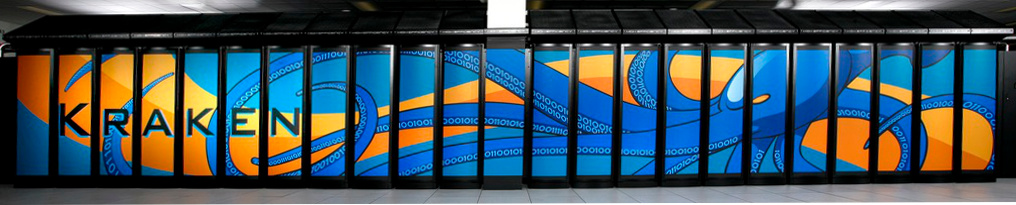
\includegraphics{../common/pics/krakenWide}
  \end{block}
\end{frame}

\begin{frame}[fragile]
  \begin{block}{pbdDMAT Scalability Benchmarks}
    \begin{minipage}{0.44\textwidth}
      \vspace{-3ex}
      \begin{lstlisting}
x <- ddmatrix("rnorm", nrow=n, ncol=p)
cov.x <- cov(x)
      \end{lstlisting}
      \vspace{-3ex}
      \begin{center}
        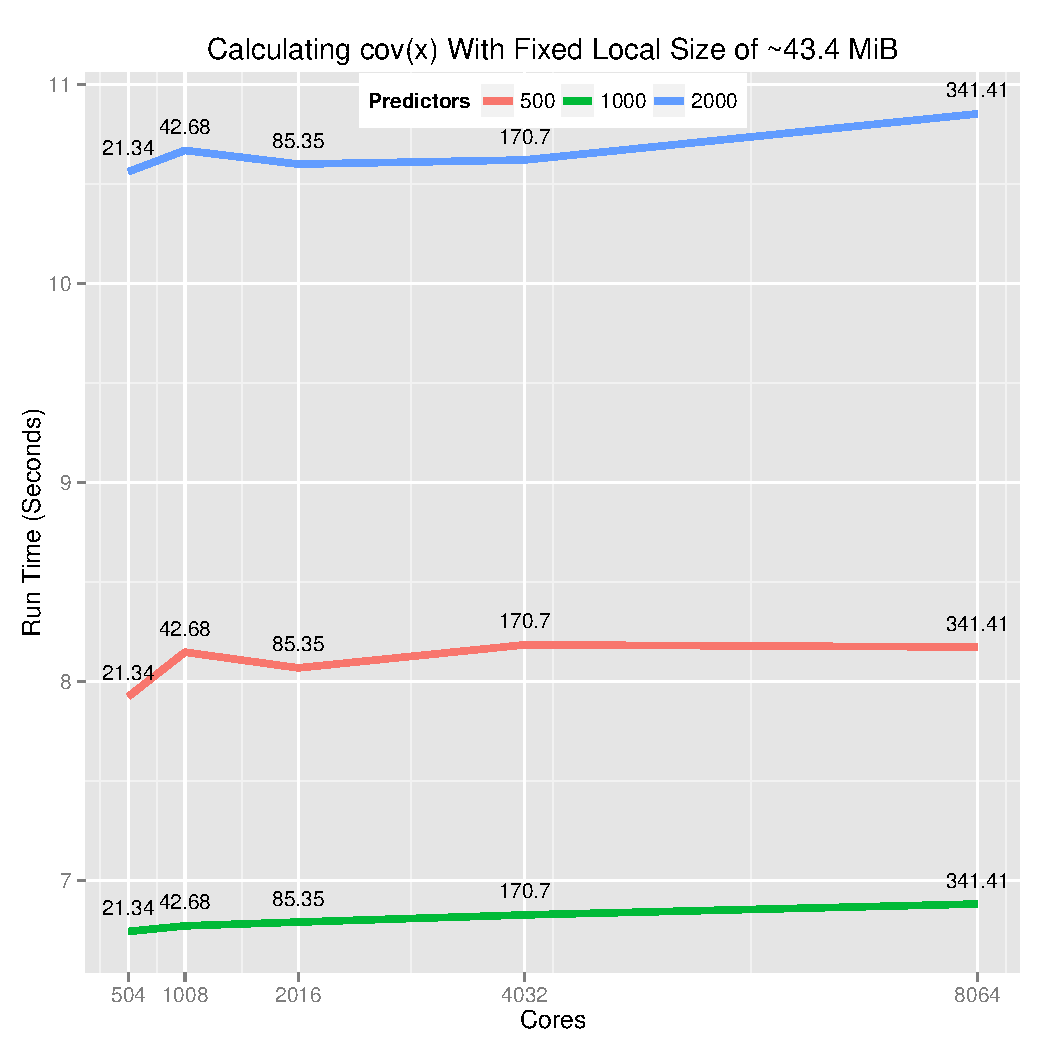
\includegraphics[trim=3mm 1mm 2mm 11.5mm,clip,width=.98\textwidth]{../common/pics/cov}
      \end{center}
    \end{minipage}
%    \hspace{.01ex}
    \begin{minipage}{0.55\textwidth}
      \vspace{-3.5ex}
      \begin{lstlisting}
b <- ddmatrix("runif", nrow=p, ncol=1)
y <- x %*% b
b.hat <- lm.fit(x, y)$coefficients
      \end{lstlisting} %$
      \vspace{-3ex}
      \begin{center}
        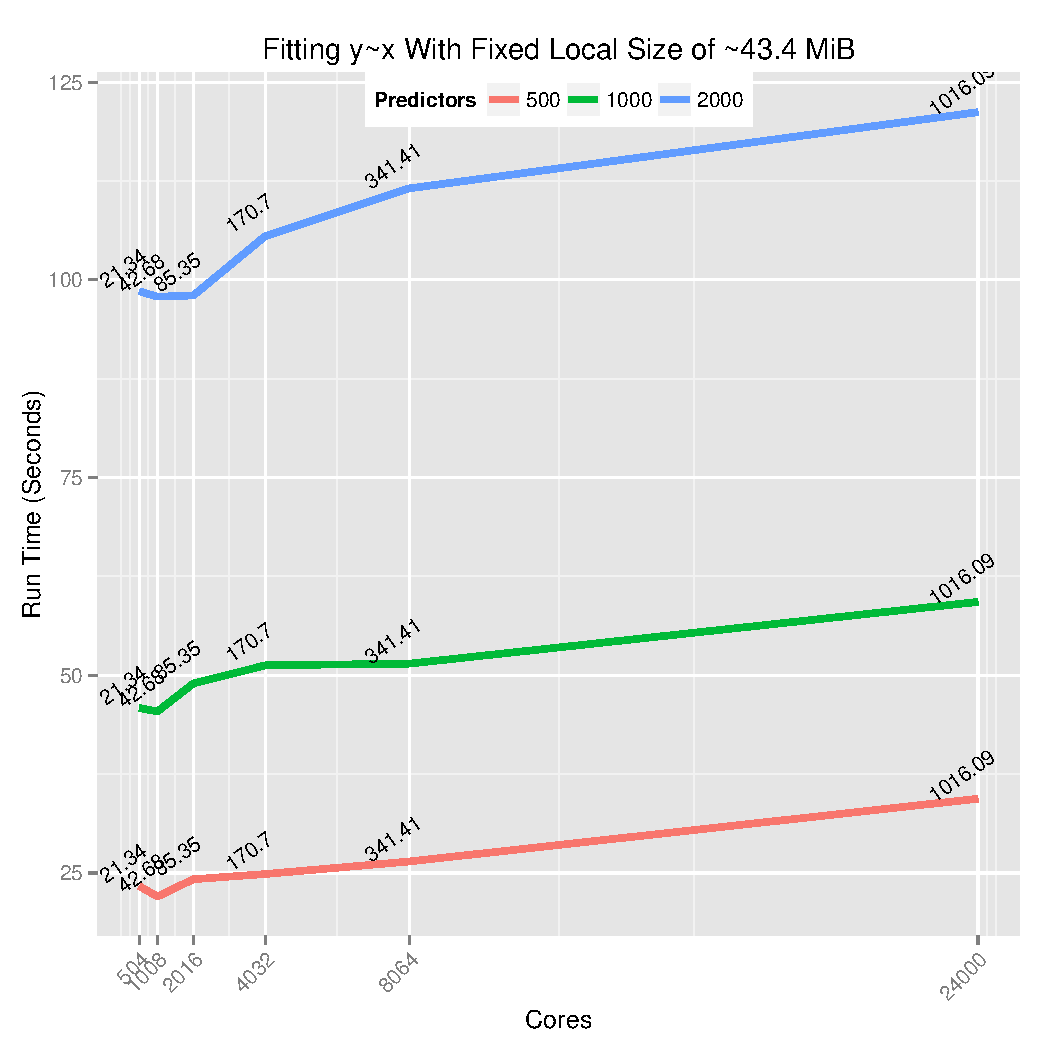
\includegraphics[trim=3mm 1mm 2mm
        12mm,clip,width=.98\textwidth]{../common/pics/benchmarks/lmfit2}
      \end{center}
    \end{minipage}
  \end{block}
\end{frame}

\begin{frame}
  \begin{block}{Matrix Exponentiation (pbdDMAT)}
    \begin{minipage}{5cm}
      \begin{itemize}\tiny
      \item Fitting biogeography models requires many matrix exponentiations
      \item Benchmark: Matrix exponential of 5000$\times$5000 matrix.
      \item R 3.1.0, Matrix 1.1-2, rexpokit 0.25, pbdDMAT 0.3-0
      \item Libs: Cray LibSci, NETLIB ScaLAPACK, Compilers: gnu 4.8.2
      \item Configuration: 1 thread == 1 MPI rank == 1 physical core
      \end{itemize}
      \vspace{-4ex}
      \begin{center}
        \includegraphics[trim=4cm 2cm 3.5cm 2.2cm,clip=true,height=4cm]{pics/Biogeography}
      \end{center}
    \end{minipage}
    \begin{minipage}{6.9cm}
      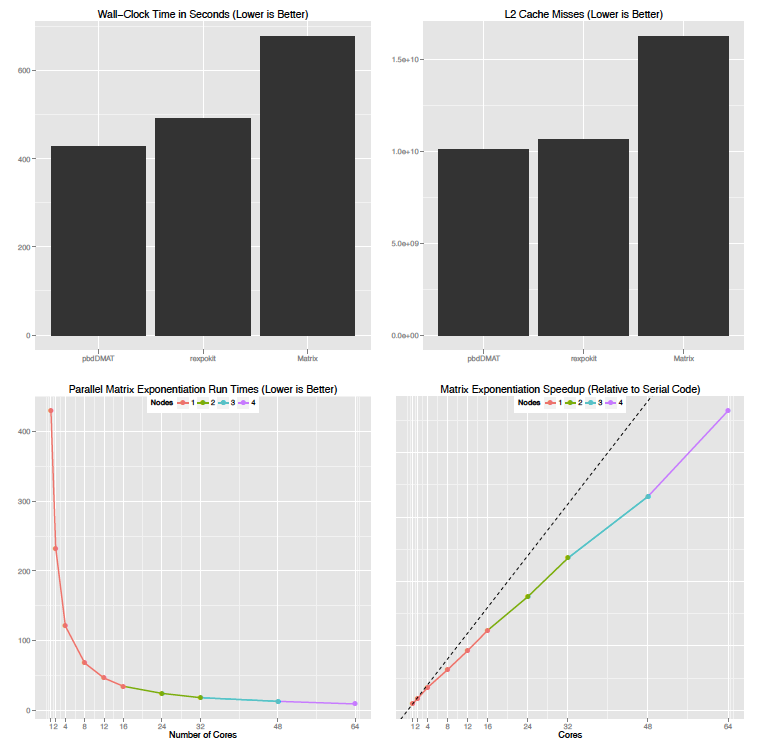
\includegraphics[trim=1mm 1mm 1mm 1mm,clip=true,height=7cm]{pics/MatExp}
    \end{minipage}
  \end{block}
  \begin{raggedright}\tiny
    Schmidt and Matzke (2014) Distributed matrix exponentiation, The R
    User Conference (UseR! 2014), \\[-2ex] Los Angeles, CA, August 2014 .
  \end{raggedright}
\end{frame}

\subsection{RandSVD}
\makesubcontentsslidessec


\begin{frame}[fragile]
\fontsize{8pt}{10}\selectfont
\begin{block}{Randomized truncated SVD\footnotemark}
  \begin{minipage}{.56\textwidth}
    \begin{center}
      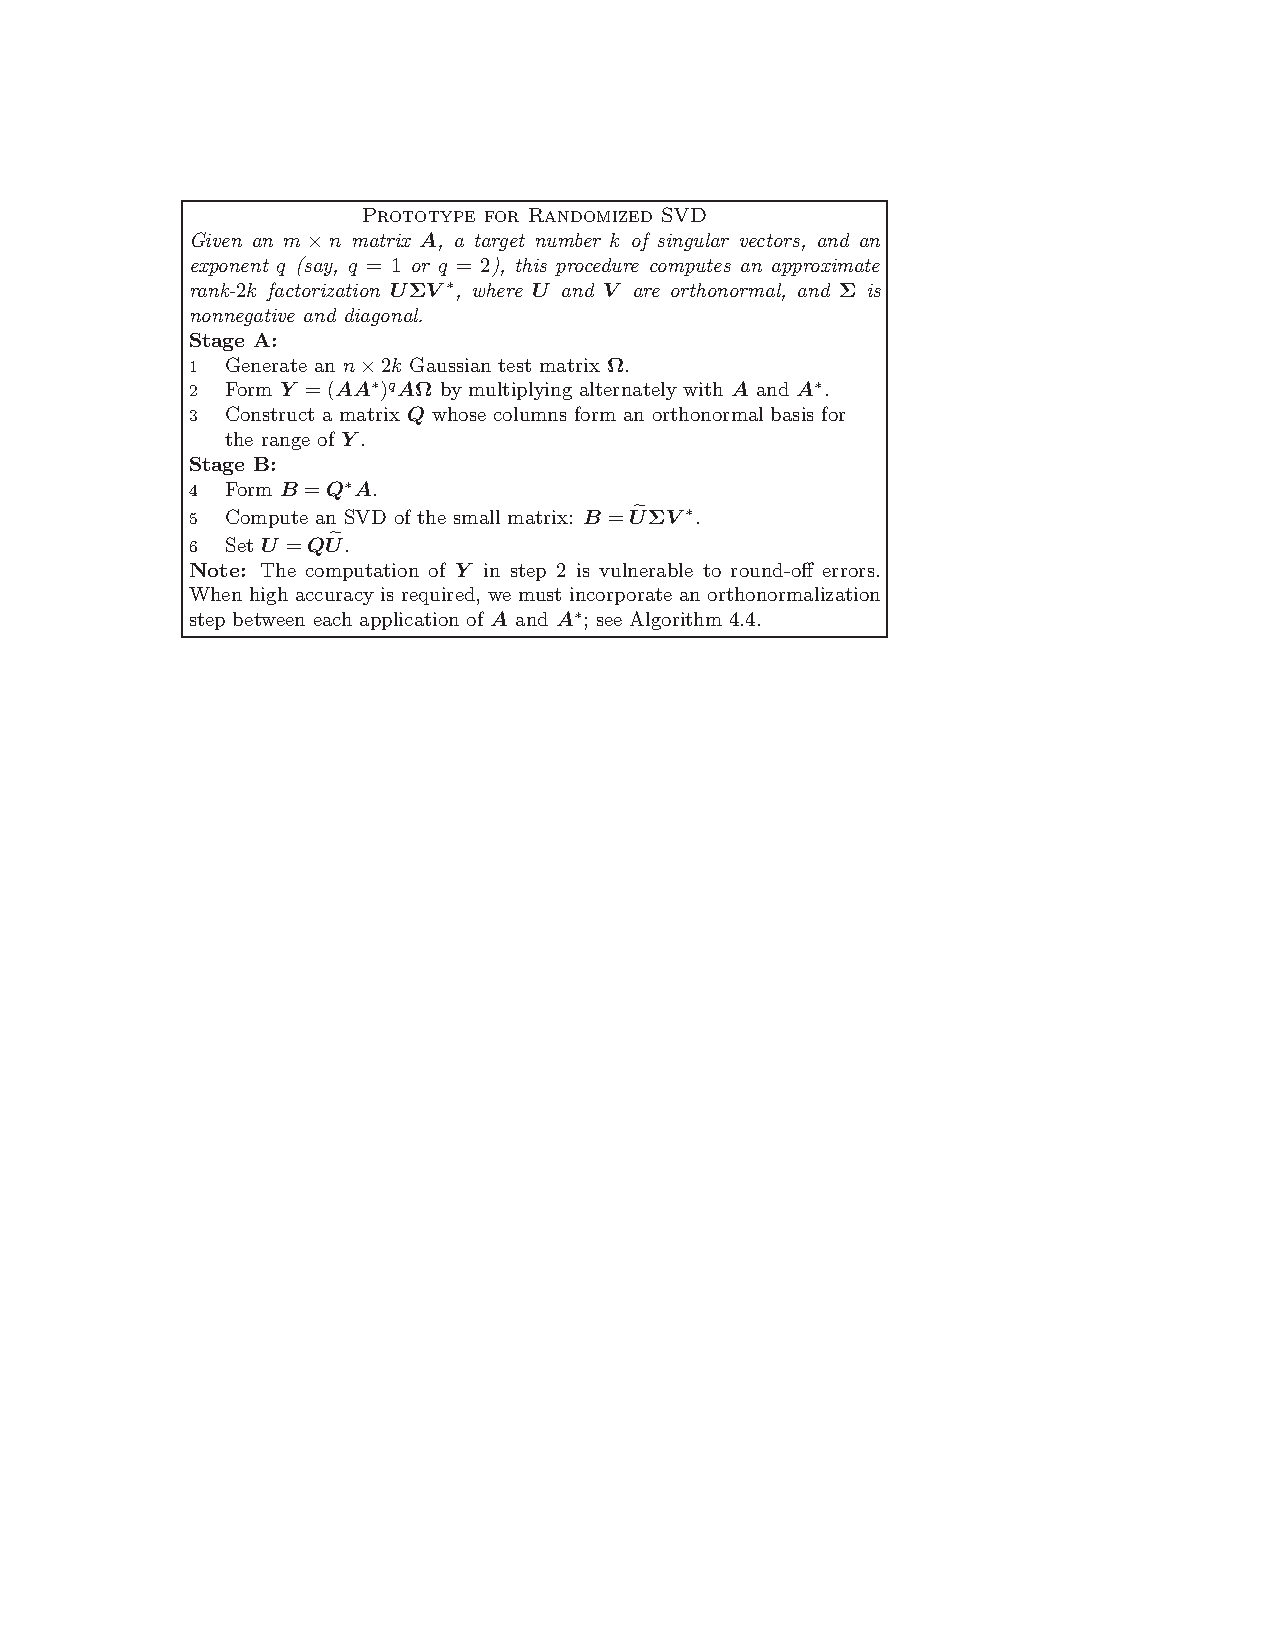
\includegraphics[height=.41\textheight]{../common/pics/randsvd/randSVDalg}
      \\
      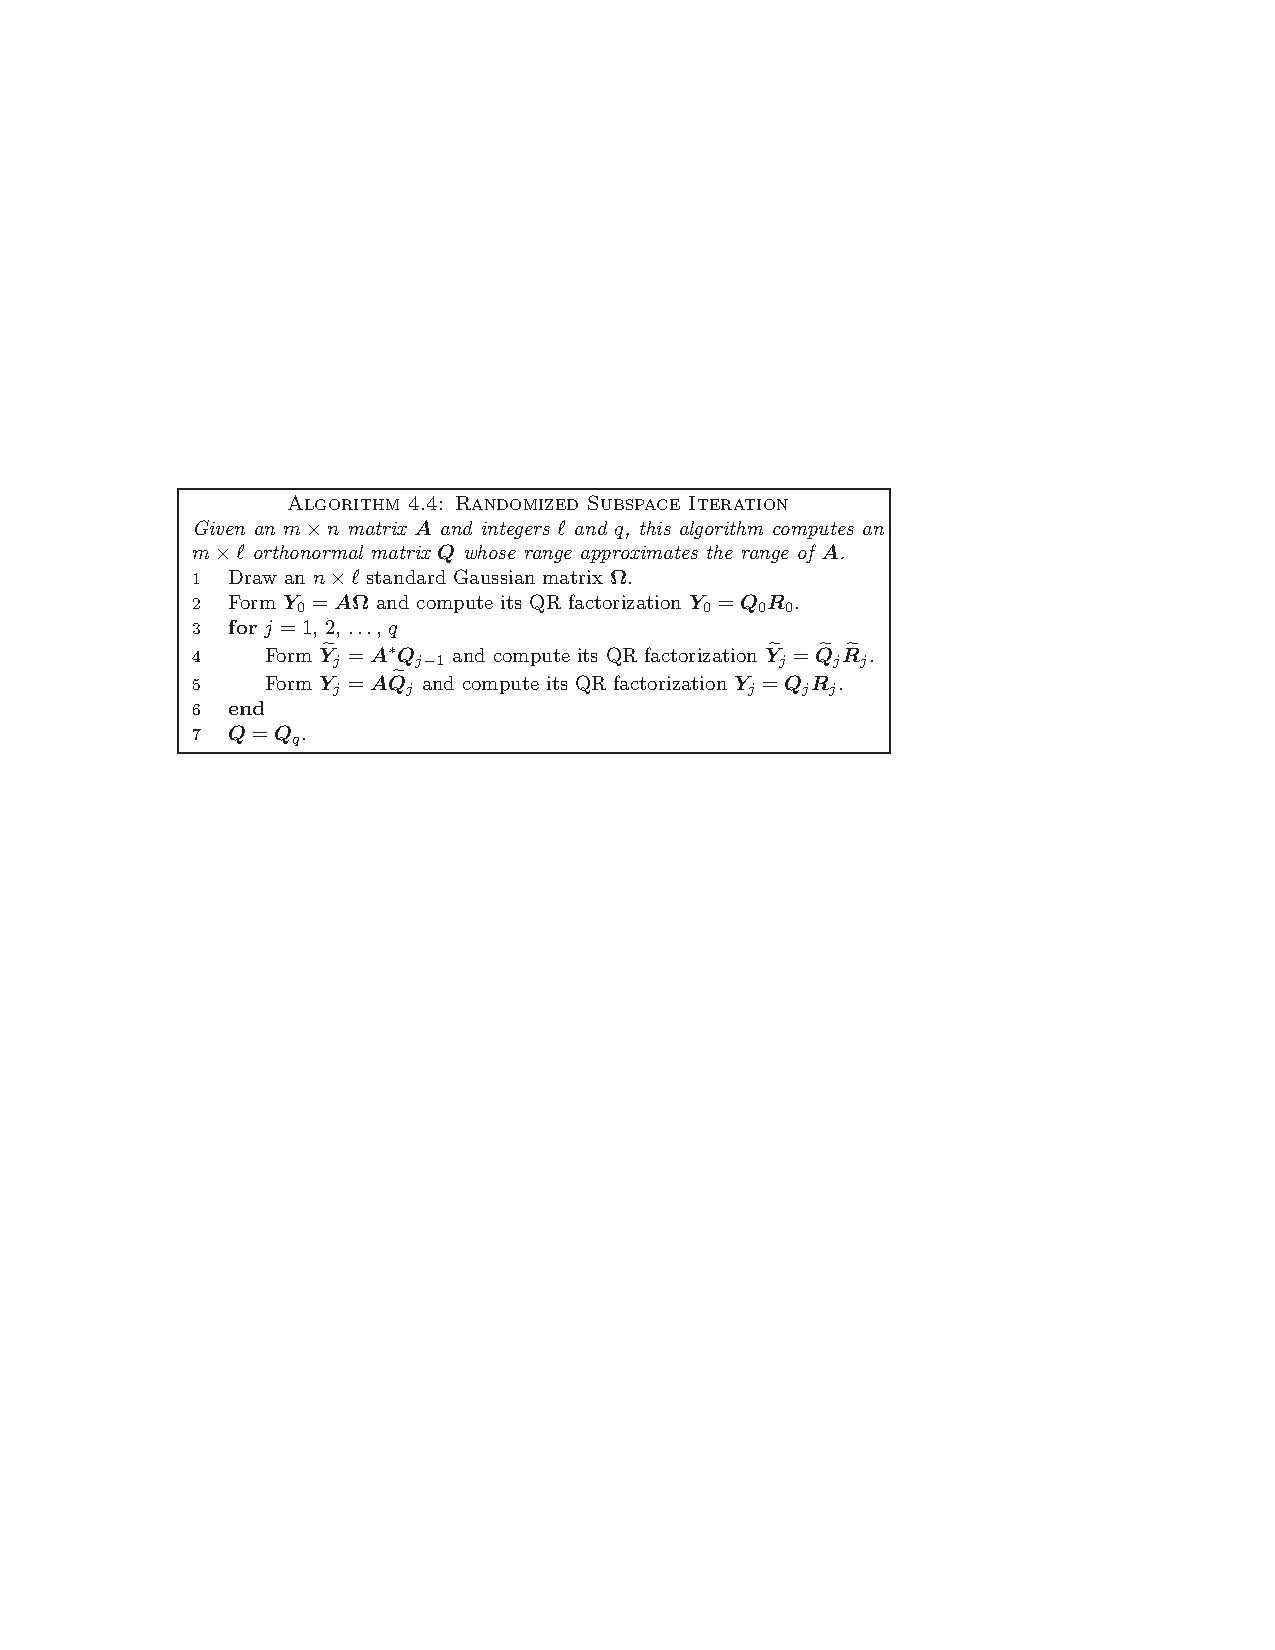
\includegraphics[height=.26\textheight]{../common/pics/randsvd/randSVDalg4_4}
    \end{center}
  \end{minipage}
%   \hspace{.01cm}
  \begin{minipage}{0.43\textwidth}
\begin{lstlisting}[title=Serial 
R,basicstyle=\tiny,backgroundcolor=\color{grayish} 
,numberstyle=\tiny\color{black},keywordstyle=\color{black},commentstyle=\color{ 
dkgreen},stringstyle=\color{black},escapeinside={(*@}{@*)}]
randSVD <- function(A, k, q=3)
  {
    ## Stage A
    Omega <- (*@ matrix(rnorm(n*2*k),@*)
      (*@ nrow=n, ncol=2*k) @*)
    Y <- A %*% Omega
    Q <- qr.Q(qr(Y))
    At <- t(A)
    for(i in 1:q)
      {
        Y <- At %*% Q
        Q <- qr.Q(qr(Y))
        Y <- A %*% Q
        Q <- qr.Q(qr(Y))
      }
    
    ## Stage B
    B <- t(Q) %*% A
    U <- La.svd(B)$u
    U <- Q %*% U
    U[, 1:k]
  }
\end{lstlisting} %balance$
\end{minipage}
{\fontsize{6pt}{10}\selectfont $^1$Halko, Martinsson, 
  and Tropp. 2011. Finding structure with randomness: probabilistic
  algorithms  for constructing \\[-1ex] approximate matrix decompositions
  \emph{SIAM Review} \textbf{53} 217--288}
\end{block}
\end{frame}


\begin{frame}[fragile]
 \fontsize{8pt}{10}\selectfont
\begin{block}{Randomized truncated SVD}
  \hfill
  \begin{minipage}{0.430\textwidth}
\begin{lstlisting}[title=Serial 
R,basicstyle=\tiny,backgroundcolor=\color{grayish} 
,numberstyle=\tiny\color{black},keywordstyle=\color{black},commentstyle=\color{ 
dkgreen},stringstyle=\color{black},escapeinside={(*@}{@*)}]
randSVD <- function(A, k, q=3)
  {
    ## Stage A
    Omega <- (*@ \textcolor{blue}{matrix(rnorm(n*2*k),} @*)
      (*@ \textcolor{blue}{ nrow=n, ncol=2*k)} @*)
    Y <- A %*% Omega
    Q <- qr.Q(qr(Y))
    At <- t(A)
    for(i in 1:q)
      {
        Y <- At %*% Q
        Q <- qr.Q(qr(Y))
        Y <- A %*% Q
        Q <- qr.Q(qr(Y))
      }
    
    ## Stage B
    B <- t(Q) %*% A
    U <- La.svd(B)$u
    U <- Q %*% U
    U[, 1:k]
  }
\end{lstlisting} %balance$
  \end{minipage}
  \hfill
  \begin{minipage}{0.430\textwidth}
\begin{lstlisting}[title=Parallel pbdR,basicstyle=\tiny,backgroundcolor=\color{
grayish}, numberstyle=\tiny\color{black},keywordstyle=\color{black},
commentstyle=\color{dkgreen},stringstyle=\color{black},escapeinside={(*@}{@*)}]
randSVD <- function(A, k, q=3)
  {
    ## Stage A
    Omega <- (*@ \textcolor{blue}{ddmatrix("rnorm",} @*)
      (*@ \textcolor{blue}{nrow=n, ncol=2*k)} @*)
    Y <- A %*% Omega
    Q <- qr.Q(qr(Y))
    At <- t(A)      
    for(i in 1:q)
      {
        Y <- At %*% Q   
        Q <- qr.Q(qr(Y))
        Y <- A %*% Q    
        Q <- qr.Q(qr(Y))
      }
    
    ## Stage B
    B <- t(Q) %*% A     
    U <- La.svd(B)$u 
    U <- Q %*% U     
    U[, 1:k]
  }
\end{lstlisting}  % balancing $
  \end{minipage}
\hfill
\end{block}
\end{frame}

\begin{frame}
  \begin{block}{From journal to scalable code and scaling data in one day.}
    \begin{center}
      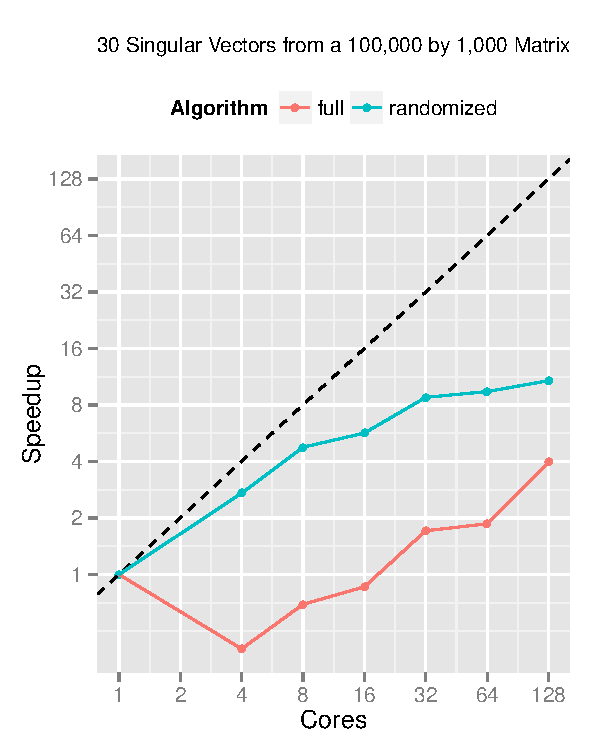
\includegraphics[width=.4\textwidth]{../common/pics/randsvd/randSVDspeedup}
      \hspace{1cm}
      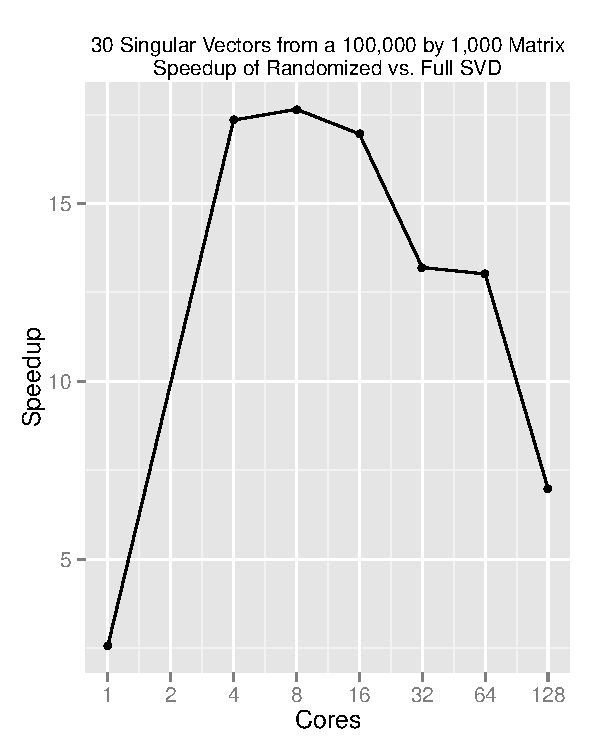
\includegraphics[width=.4\textwidth]{../common/pics/randsvd/randSpeedupSVD}
    \end{center}
  \end{block}
\end{frame}

\subsection{pbdMPI Example: Random Forest Prediction}
\makesubcontentsslidessec


\begin{frame}[fragile]{Letter Recognition Data}
  \begin{exampleblock}{Example \countex : Letter Recognition data from
      package \pkg{mlbench} (20,000 $\times$ 17)}\pause
    \vspace{-1em}
    \begin{minipage}{0.3\textwidth}
      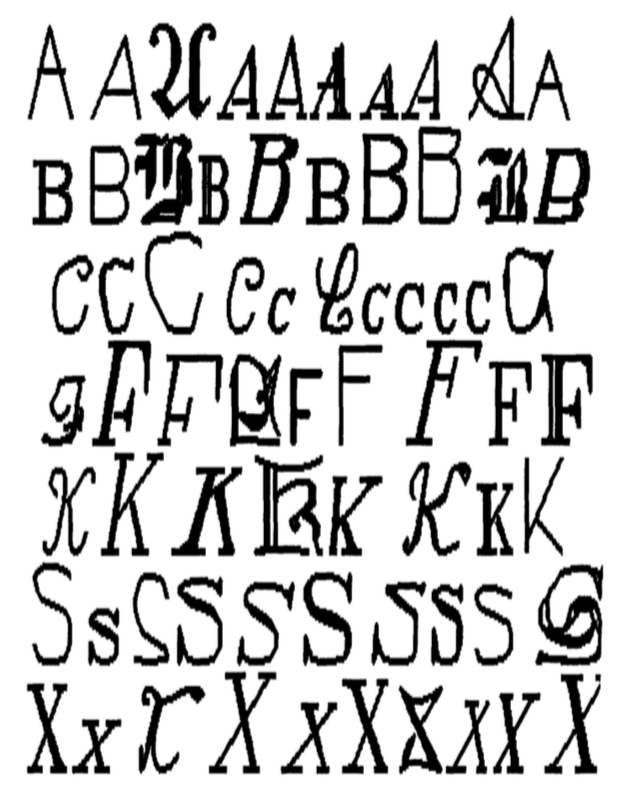
\includegraphics[width=0.95\textwidth]{../common/pics/apps/ML_FreySlate1991}
    \end{minipage}
    \begin{minipage}{0.69\textwidth}\tiny
      \begin{lstlisting}
[,1]	lettr	capital letter
[,2]	x.box	horizontal position of box
[,3]	y.box	vertical position of box
[,4]	width	width of box
[,5]	high	height of box
[,6]	onpix	total number of on pixels
[,7]	x.bar	mean x of on pixels in box
[,8]	y.bar	mean y of on pixels in box
[,9]	x2bar	mean x variance
[,10]	y2bar	mean y variance
[,11]	xybar	mean x y correlation
[,12]	x2ybr	mean of x^2 y
[,13]	xy2br	mean of x y^2
[,14]	x.ege	mean edge count left to right
[,15]	xegvy	correlation of x.ege with y
[,16]	y.ege	mean edge count bottom to top
[,17]	yegvx	correlation of y.ege with x
      \end{lstlisting}
    \end{minipage} \\
    {\tiny P. W. Frey and D. J. Slate (Machine Learning Vol 6/2 March 91):
    "Letter Recognition Using Holland-style Adaptive Classifiers".}
  \end{exampleblock}
\end{frame}


\begin{frame}
  \begin{exampleblock}{Example \showex : Random Forest Algorithm}\pause
    \begin{enumerate}
     \item Build simple regression trees from random subsets of
       columns
     \item Use model averaging for prediction
     \item Package \pkg{randomForest} has a \code{combine} function
       \begin{enumerate}
       \item Everyone gets the same training data
       \item Split regression tree building among processors
       \item Use \code{allgather} to bring built predictors to all
       \item Everyone \code{combine} predictors
       \item Split prediction work by blocks of rows
       \item Use \code{allreduce} to assess prediction
       \end{enumerate}
     \item Steps (3) and (4) can be improved with a custom
       reduce/combine to take advantage of MPI vendor optimizations
    \end{enumerate}
  \end{exampleblock}
\end{frame}


\begin{frame}[fragile]
  \begin{exampleblock}{Example \showex :  Random Forest Code \\
      (Split learning by blocks of trees. Split prediction by blocks
      of rows.)}\pause
    \begin{lstlisting}[title=Serial Code]
data(LetterRecognition) # 26 Capital Letters Data 20,000 x 17
set.seed(seed=1234567)
n <- nrow(LetterRecognition)
## get train data
n_train <- floor(0.8*n)
i_train <- sample.int(n, n_train) # Use 4/5 of the data to train
train <- LetterRecognition[i_train, ]
test <- LetterRecognition[-i_train, ]

## train random forest
my.k <- 500
rf.all <- randomForest(lettr ~ ., train, ntree=my.k, norm.votes=FALSE)

## predict test data
pred <- predict(rf.all, test)
correct <- sum(pred == test$lettr)
cat("Proportion Correct:", correct/(n - n_train), "\n")
    \end{lstlisting} %$
  \end{exampleblock}
\end{frame}


\begin{frame}[fragile]
  \begin{exampleblock}{Example \showex :  Random Forest Code \\
      (Split learning by blocks of trees. Split prediction by blocks
      of rows.)}\pause
    \begin{lstlisting}[title=Parallel Code,escapeinside={(*@}{@*)}]
data(LetterRecognition) # 26 Capital Letters Data 20,000 x 17
(*@\textcolor{red}{comm.}@*)set.seed(seed=123(*@\textcolor{red}{, diff=FALSE}@*)) # same training data
n <- nrow(LetterRecognition)
n_train <- floor(0.8*n)
i_train <- sample.int(n, n_train) # Use 4/5 of the data to train
train <- LetterRecognition[i_train, ]
(*@\textcolor{red}{my.test\_rows <- get.jid(n - n\_train)}@*)  # different test data
test <- LetterRecognition[-i_train, ](*@\textcolor{red}{[my.test\_rows, ]}@*)

(*@\textcolor{red}{comm.}@*)set.seed(seed=1e6*runif(1)(*@\textcolor{red}{, diff=TRUE}@*))
my.k <- floor(500(*@\textcolor{red}{/comm.size()}@*))
my.rf <- randomForest(lettr ~ ., train, ntree=my.k, norm.votes=FALSE)

(*@\textcolor{red}{rf.each <- allgather(my.rf)}@*)
(*@\textcolor{red}{rf.all <- do.call(combine, rf.each)}@*)

pred <- predict(rf.all, test)
correct <- (*@\textcolor{red}{allreduce(}@*)sum(pred == test\$lettr)(*@\textcolor{red}{)}@*)
(*@\textcolor{red}{comm.}@*)cat("Proportion Correct:", correct/(n - n_train), "\n")
    \end{lstlisting} %$
  \end{exampleblock}
\end{frame}

\subsection{pbdMPI Example: Functional Data Analysis}
\makesubcontentsslidessec


\begin{frame}[fragile]{fda.usc Package}
  \begin{block}{Profiling min.basis()}\pause
    \vspace{-2ex}
    \begin{lstlisting}[escapeinside={(*@}{@*)}]
> summaryRprof()
$by.total
                     total.time total.pct self.time self.pct
"min.basis"               12.32    100.00      0.00     0.00
"type.CV"                  6.54     (*@\color{red}{53.08 }@*)      0.02     0.16
"S.basis"                  5.76     (*@\color{red}{46.75 }@*)      0.00     0.00
"drop"                     4.20     34.09      0.00     0.00
"norm.fdata"               4.20     34.09      0.00     0.00
"metric"                   4.18     33.93      1.04     8.44
"%*%"                      3.98     32.31      3.98    32.31
"getbasispenalty"          2.72     22.08      0.02     0.16
"bsplinepen"               2.68     21.75      0.36     2.92
"int.simpson2"             2.54     20.62      1.96    15.91
"t"                        2.10     17.05      0.10     0.81
"ppBspline"                1.60     12.99      0.82     6.66
. . .
    \end{lstlisting}
%$
  \end{block}
\end{frame}

\begin{frame}[fragile]
  \begin{block}{Example: min.basis() ~110 lines \hfill SPMD: Add 5, change 3}\pause
    \begin{lstlisting}[escapeinside={(*@}{@*)}]
min.basis <- function(fdataobj, type.CV = GCV.S, . . ., ...)
{
    . . . 13 lines
    (*@\color{red}{library(pbdMPI)}@*)
    (*@\color{red}{init()}@*)
    (*@\color{red}{my.k <- get.jid(lenlambda)}@*)
    my.gcv <- array(Inf, dim = c(lenbasis, (*@\color{red}{length(my.k)}@*)))
    . . . 36 lines
    for (i in 1:lenbasis) {
        . . . 3 lines
        for (k in (*@\color{red}{my.k}@*)) {
            S2 <- S.basis(tt, base, lambda[k])
            (*@\color{red}{my.gcv[i, k - my.k[1] + 1]}@*) <-
                type.CV(fdataobj, S = S2, W = W, trim = par.CV$trim, draw = par.CV$draw, ...)
        }
    }
    (*@\color{red}{gcv <- do.call(cbind, allgather(my.gcv))}@*)
    (*@\color{red}{finalize()}@*)
    . . . 48 lines
    \end{lstlisting} %$
  \end{block}
\end{frame}



%\begin{frame}
  \begin{block}{An Interesting Tweet...}
    \begin{center}
      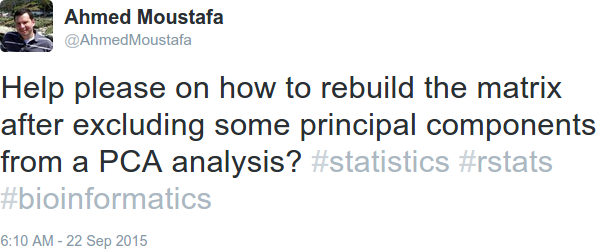
\includegraphics[width=.95\textwidth]{../common/pics/decomprecomp/tweet1}
    \end{center}
  \end{block}
\end{frame}


\begin{frame}
  \begin{block}{A Clarification}
    \begin{center}
      
\includegraphics[width=.95\textwidth]{../common/pics/decomprecomp/tweet2}
    \end{center}
  \end{block}
\end{frame}


\begin{frame}
  \begin{block}{The Idea}
    \begin{align*}
      X = U \Sigma V^T
    \end{align*}
    % TODO finish the math
  \end{block}
\end{frame}


\begin{frame}
  \begin{block}{Properties}
    Say we remove the first principal component:
    \begin{itemize}
      \item PC2 becomes PC1
      \item PC3 becomes PC2
      \item Variance of PC3 is 0.
    \end{itemize}
  \end{block}
\end{frame}


\begin{frame}
  \begin{block}{Algorithm}
    \begin{itemize}
      \item Compute SVD $X = U\Sigma V^T$ with \code{La.svd()}.
      \item Drop desired columns of $U$, $\Sigma$, and $V$.
      \item Use \code{sweep()} to multiply reduced $U$ by reduced $\Sigma$, column-wise to form $U\Sigma$.
      \item Multiply $(U\Sigma)$ on the right by reduced $V^T$.
    \end{itemize}
  \end{block}
\end{frame}



\begin{frame}[fragile]
\fontsize{8pt}{10}\selectfont
\begin{block}{Decomp-Recomp}
\begin{lstlisting}[title=Serial And Parallel]
decomp_recomp <- function(x, exclude, center=TRUE, scale=FALSE)
{
  if (center || scale)
    x <- scale(x, center=center, scale=scale)
  
  svd <- La.svd(x)
  
  u <- svd$u
  d <- svd$d
  vt <- svd$vt
  
  ud <- sweep(u[, -exclude], MARGIN=2, FUN="*", STAT=d[-exclude])
  ud %*% vt[-exclude, ]
}
\end{lstlisting}
\end{block}
\end{frame}



